% This is samplepaper.tex, a sample chapter demonstrating the
% LLNCS macro package for Springer Computer Science proceedings;
% Version 2.20 of 2017/10/04
%
\documentclass[runningheads]{llncs}
%
\usepackage{graphicx}
% Used for displaying a sample figure. If possible, figure files should
% be included in EPS format.
%
% If you use the hyperref package, please uncomment the following line
% to display URLs in blue roman font according to Springer's eBook style:
% \renewcommand\UrlFont{\color{blue}\rmfamily}
\usepackage{hyperref}

\begin{document}
%
\title{Music streaming and song recommendations using ML algorithms}
%
%\titlerunning{Abbreviated paper title}
% If the paper title is too long for the running head, you can set
% an abbreviated paper title here
%
\author{Anthony M. Schomer}
%
\authorrunning{A. Schomer.}
% First names are abbreviated in the running head.
% If there are more than two authors, 'et al.' is used.
%
\institute{Northwest Missouri State University, Maryville MO 64468, USA \\
\email{tony.schomer@gmail.com}}
%
\maketitle              % typeset the header of the contribution
%
\begin{abstract}
This capstone project investigates the algorithms used by music streaming services to recommend similar songs to enhance user experiences. The focus is on how platforms like Spotify and Apple Music use listeners preferences including Likes, dislikes, and other relevant information to create personalized playlists tailored to individual tastes. This project uses open datasets such as Spotify Million Playlist Dataset, Spotify Web API, and Musicbrain.org's extensive library of databases. Using smart computer programs to create a test system that suggests songs based on user behavior and preferences. It looks at how current song recommendations systems work. Machine learning methods. such as, collaborative filtering and content-based analysis to build test recommendation systems. This project also will address challenges within the current algorithms to help avoid common issues. One significant issue to avoid is users hearing the same song over and over again. These findings will help improve the music discovery online and suggest ways to innovate and enhance recommendations for listeners and introduce them to new artists. 

\keywords{music \and streaming \and recommendations \and data \and user experience}
\end{abstract}
%
%
%
\section{Introduction}

Listening to music is something many people do daily. Whether it is at the gym, at work, commuting from place to place. Most people use their phones to access streaming music services.   The first paragraph that follows a table, figure,
equation etc. does not need an indent, either.

Subsequent paragraphs, however, are indented.

\subsection{Goals of this Research} 
 How music streaming services use algorithms to recommend similar songs to users. 
 Analyzing the processes of recommendations, the goal is to understand how these platforms personalize playlists and suggest new music that is similar to what the listeners' would enjoy..

\subsection{The following are the phases of implementation for the Project}
\begin{enumerate}
\item Research and Data Collection
    \begin{enumerate}
        \item Study existing music streaming platforms, Spotify, Apple Music).
        \item Gather open datasets (Spotify Million Playlist Datasets, Spotify Web API, Musicbrainz.org).
        \item Analyze user behavior data and song characteristics.
    \end{enumerate}
\item Algorithm Analysis
    \begin{enumerate}
        \item Examine current song recommendation systems and identify key factors influencing recommendations. 
        \item Study collaborative filtering and content-based analysis techniques. 
    \end{enumerate}
\item Development of Test System
    \begin{enumerate}
        \item Design and implement a prototype recommendation system using machine learning methods. 
        \item Integrate user behavior and preferences into the system. 
    \end{enumerate}
\item Addressing Possible Challenges
    \begin{enumerate}
        \item Develop strategies to enhance recommendation variety and avoid songs playing over and over. 
    \end{enumerate}
\item Analysis and Conclusion
    \begin{enumerate}
        \item Interpret findings from the test system and develop suggestions to improve music discovery.
        \item Discuss implications for listeners and new artists. 
    \end{enumerate}
\item Final Report and Presentation
    \begin{enumerate}
        \item Compile research and present findings and music streaming recommendations.
    \end{enumerate}
\end{enumerate}


\section{Popular Music Styles and Tables}

\begin{figure}
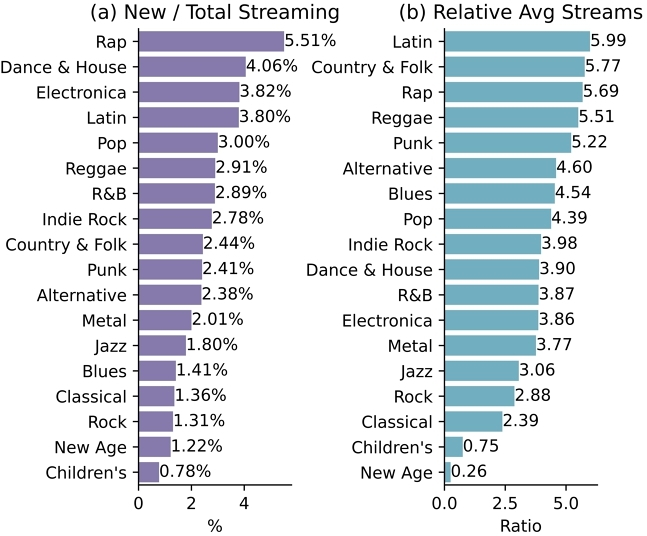
\includegraphics[width=\textwidth]{streaming 2.jpg}
\caption{This table shows the difference between New Streaming to Average Streams.} 
\label{fig1}
\end{figure}

\begin{figure}
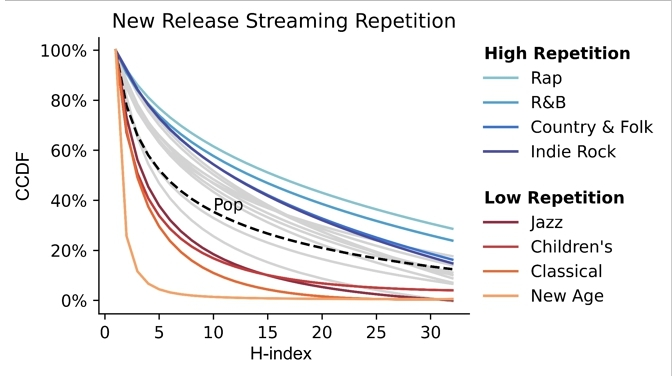
\includegraphics[width=\textwidth]{Streaming 1.jpg}
\caption{This is New Release Streaming Repetition} 
\label{mecFig}
\end{figure}

%\begin{theorem}
%This is a sample theorem. The run-in heading is set in bold, while
%the following text appears in italics. Definitions, lemmas,
%propositions, and corollaries are styled the same way.
%\end{theorem}
%
% the environments 'definition', 'lemma', 'proposition', 'corollary',
% 'remark', and 'example' are defined in the LLNCS documentclass as well.
%


The following items might help algorithm find new musicians for users:
\begin{itemize}
    \item Style
    \item bass
    \item tempo
    \item genre
    \item tour lineup
    \item single artist
    \item group
\end{itemize}
    

% ---- Bibliography ----
%
% BibTeX users should specify bibliography style 'splncs04'.
% References will then be sorted and formatted in the correct style.
%
\bibliographystyle{splncs04}
\bibliography{mybibliography}

\href{https://www.kaggle.com/code/caitlyna/music-database-analysis}{Kaggle: Music Database Analysis}

\href{https://dl.acm.org/doi/fullHtml/10.1145/3614419.3644002}{ACM: Music Streaming Paper}

\href{https://developer.spotify.com/documentation/web-api}{Spotify Web API Documentation}

\href{https://musicbrainz.org/}{MusicBrainz}

\href{https://www.overleaf.com/project/671af4c6d1ae0a41998555c6}{Overleaf Project}

\href{https://github.com/anythonyschomer/capstoneproject}{GitHub Repository}

\end{document}